\textbf{COLUNI 2018 -- Questão 38}\par\medskip A descolonização afro-asiática é um dos efeitos mais marcantes das duas grandes guerras mundiais e das crises que elas causaram. As imagens, abaixo, referem-se a personalidades e às realidades sociopolíticas relacionadas ao processo de descolonização das novas nações que se formaram.

\par

\begin{center}
\begin{minipage}{0.48\linewidth}
\centering
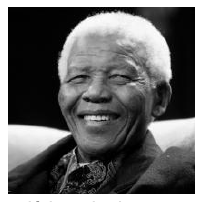
\includegraphics[width=0.72\linewidth,trim=0 12pt 0 0,clip]{static/simulados/coluni/figuras/2018/questao-38/figura-1.png}\par
Nelson Mandela, líder da luta contra o Apartheid na África do Sul\par
(Fonte: http://culturevie.info/tag-nelson-mandela.html)
\end{minipage}\hfill
\begin{minipage}{0.48\linewidth}
\centering
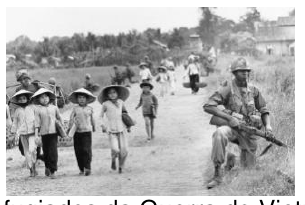
\includegraphics[width=0.88\linewidth,trim=0 12pt 0 0,clip]{static/simulados/coluni/figuras/2018/questao-38/figura-2.png}\par
Refugiados da Guerra do Vietnã\par
(Fonte: http://numaznews.blogspot.com.br/2012/08/a-guerra-do-vietna-um-pesadelo-para-os.html)
\end{minipage}\par\medskip
\begin{minipage}{0.48\linewidth}
\centering
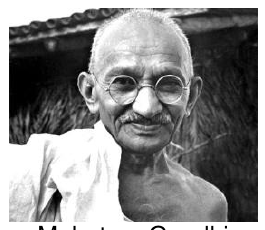
\includegraphics[width=0.78\linewidth,trim=0 12pt 0 0,clip]{static/simulados/coluni/figuras/2018/questao-38/figura-3.png}\par
Mahatma Gandhi\par
(Fonte: https://edukavita.blogspot.com.br/2015/07/biografia-de-mahatma-gandhi-arquiteto.html)
\end{minipage}\hfill
\begin{minipage}{0.48\linewidth}
\centering
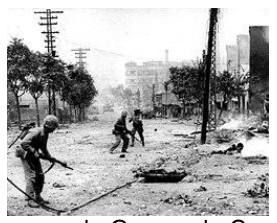
\includegraphics[width=0.82\linewidth,trim=0 12pt 0 0,clip]{static/simulados/coluni/figuras/2018/questao-38/figura-4.png}\par
Imagens da Guerra da Coreia\par
(Fonte: https://pt.wikipedia.org/wiki/Guerra\_da\_Coreia)
\end{minipage}
\end{center}

Sobre o processo histórico da descolonização e suas repercussões para a África do Sul, o Vietnã, a Índia e a Coreia, é CORRETO afirmar:


\begin{enumerate}
\item A península coreana, de possessão japonesa até 1945, foi dividida em duas repúblicas, uma capitalista ao sul
      e outra socialista ao norte. Mais tarde, a Guerra da Coreia (1950-1953) colocou as duas nações em confronto.
      Um armistício encerrou o conflito, mas a tensão permanece até a atualidade.
\item O Vietnã ficou independente da França, depois da Conferência de Genebra, em 1954, estabelecendo-se uma
      única república liberal de orientação capitalista. Nos anos 1960, os EUA invadiram o país a fim de impedir a
      expansão do domínio socialista chinês na região.
\item A África do Sul, libertada em 1947 do domínio inglês, tornou-se uma referência de nação democrática e
      inclusiva de negros e brancos, com Nelson Mandela, seu primeiro presidente pós-independência.
\item A Índia ficou independente da Inglaterra em 1947, depois de um amplo processo de luta armada, em que se
      destacou a figura de Mahatma Gandhi e seu método da desobediência civil.\end{enumerate}
